%%%%%%%%%%%%%%%%%%%%%%%%%%%%%
% Standard header for working papers
%
% WPHeader.tex
%
%%%%%%%%%%%%%%%%%%%%%%%%%%%%%

\documentclass[11pt]{article}

%%%%%%%%%%%%%%%%%%%%
%% Include general header where common packages are defined
%%%%%%%%%%%%%%%%%%%%

% general packages without options
\usepackage{amsmath,amssymb,bbm}




%%%%%%%%%%%%%%%%%%%%
%% Idem general commands
%%%%%%%%%%%%%%%%%%%%
%% Commands

\newcommand{\noun}[1]{\textsc{#1}}


%% Math

% Operators
\DeclareMathOperator{\Cov}{Cov}
\DeclareMathOperator{\Var}{Var}
\DeclareMathOperator{\E}{\mathbb{E}}
\DeclareMathOperator{\Proba}{\mathbb{P}}

\newcommand{\Covb}[2]{\ensuremath{\Cov\!\left[#1,#2\right]}}
\newcommand{\Eb}[1]{\ensuremath{\E\!\left[#1\right]}}
\newcommand{\Pb}[1]{\ensuremath{\Proba\!\left[#1\right]}}
\newcommand{\Varb}[1]{\ensuremath{\Var\!\left[#1\right]}}

% norm
\newcommand{\norm}[1]{\| #1 \|}


% amsthm environments
\newtheorem{definition}{Definition}



%% graphics

% renew graphics command for relative path providment only ?
%\renewcommand{\includegraphics[]{}}








% geometry
\usepackage[margin=2cm]{geometry}

% layout : use fancyhdr package
\usepackage{fancyhdr}
\pagestyle{fancy}

\makeatletter

\renewcommand{\headrulewidth}{0.4pt}
\renewcommand{\footrulewidth}{0.4pt}
%\fancyhead[RO,RE]{\textit{Working Paper}}
\fancyhead[RO,RE]{\textit{ECTQG 2015}}
%\fancyhead[LO,LE]{G{\'e}ographie-Cit{\'e}s/LVMT}
\fancyhead[LO,LE]{An Algorithmic Systematic Review}
\fancyfoot[RO,RE] {\thepage}
\fancyfoot[LO,LE] {\noun{J. Raimbault}}
\fancyfoot[CO,CE] {}

\makeatother


%%%%%%%%%%%%%%%%%%%%%
%% Begin doc
%%%%%%%%%%%%%%%%%%%%%

\begin{document}







\title{Models Coupling Urban Growth and Transportation Network Growth : An Algorithmic Systematic Review Approach\\\medskip
\textit{ECTQG 2015, Bari}}
\author{\noun{Juste Raimbault}$^{1,2}$\\
$^{1}$ UMR CNRS 8504 - G{\'e}ographie-Cit{\'e}s, Paris, France\\
$^{2}$ UMR-T IFSTTAR 9403 - LVMT, Champs-sur-Marne, France
}
\date{}

\maketitle

\justify

\begin{abstract}
Taking as an object of study the co-evolution of land-use and transportation infrastructure, a broad bibliographical study suggests the quasi-absence of quantitative models of simulation that would integrate both network and urban growth. This absence may be due to scientific disciplines involved that do not easily interact and are rather self-centered. We propose an algorithmic systematic review to give quantitative elements of answer to this question. A formal algorithm to retrieve corpuses of references from initial keywords, based on text-mining, is developed and implemented. We study its convergence properties and do a sensitivity analysis. We then apply it on queries typically representative of our question, and the study of retrieved corpuses tends to confirm the hypothesis.
\end{abstract}



%%%%%%%%%%%%%%%%%%%%
\section{Introduction}
%%%%%%%%%%%%%%%%%%%%

Transportation networks and urban land-use are known to be strongly coupled components of urban systems at many scales~\cite{bretagnolle:tel-00459720}. One common approach is to consider them as co-evolving rather than misleading interpretations such as the dangerous \emph{myth of structuring effect of transportation}~\cite{offner1993effets}. A question rapidly arising is the existence of models that endogeneize this co-evolution, taking into account simultaneously urban and network growth. We try to answer it using an algorithmic systematic review. The rest of the paper is organized as follows : after a brief state of the art of existing literature, we present the approach and formalize the algorithm, which results are then presented and discussed.

%%%%%%%%%%%%%%%%%%%%
\subsection{Modeling Interactions between Urban Growth and Network Growth : State of the Art}

\paragraph{Land-Use Transportation Interaction Models}

A wide class of models that have been developed essentially for planning purposes, which are the so-called \emph{Land-use Transportation Interaction Models}, is a first type answering our research question. See recent reviews~\cite{chang2006models,iacono2008models,wegener2004land} to get an idea of the heterogeneity of included approaches, that exist for more than 30 years ago. Recent models with diverse refinements are still developed today, such as~\cite{delons:hal-00319087} which includes housing market for Paris area. Diverse aspects of the same system can be translated into divers models (see e.g. \cite{wegener1991one}), and traffic, residential and employment dynamics, resulting land-use evolution, influenced also by a static transportation network, are generally taken into account.

\paragraph{Network Growth Approaches}
On the contrary, many economic literature has done the opposite of previous models, i.e. trying to reproduce network growth given assumptions on the urban landscape, as reviewed in~\cite{zhang2007economics}. In~\cite{xie2009modeling}, economic empirical are positioned within other network growth approaches, such as work by physicists giving model of geometrical network growth~\cite{barthelemy2008modeling}. Analogy with biological networks was also done, reproducing typical robustness properties of transportation networks~\cite{TeroAl10}.


\paragraph{Hybrid Approaches}

Very few approaches coupling urban growth and network growth can be found in the literature. \cite{barthelemy2009co} couple density evolution with network growth in a toy model, obtaining theoretical results. In~\cite{raimbault2014hybrid}, a simple Cellular Automaton coupled with an evolutive network reproduces stylized facts of \emph{human settlements} described by \noun{Le Corbusier}. At a smaller scale, \cite{achibet2014model} proposes a model of co-evolution between roads and buildings, following geometrical rules. These approaches stay however limited and exceptional.


%%%%%%%%%%%%%%%%%%%%
\subsection{Bibliometrical Approach}

Literature review is a crucial preliminary step for any scientific work and its quality and extent may have a dramatic impact on perspectives for research question and objectives, and systematic review techniques have been developed, from qualitative review techniques to quantitative meta-analyses allowing to produce new results by combining existing studies~\cite{rucker2012network}. Missing some references can be considered as a scientific mistake in the context of emerging information systems~\cite{lissacksubliminal}. Using a systematic technique should be an advantage to tackle our issue.

Indeed, observing the form of the bibliography obtained in previous section raises some hypothesis. We see that all components are present for co-evolutive models to exist but that a lack of communication seems to impede it. As it was shown in~\cite{commenges:tel-00923682} for the concept of mobility, for which a ``small world of actors'' relatively closed invented a notion \emph{ad hoc}, using models without accurate knowledge of a more general scientific context, we could be in an analog case for the type of models we are interested in. Restricted interactions between scientific fields working on the same objects but with different purposes, backgrounds and at different scales, could be at the origin of the relative absence of co-evolving models. We propose an algorithmic method described in the following to enlighten this issue.


%%%%%%%%%%%%%%%%%%%%
\section{Description of the Algorithm}
%%%%%%%%%%%%%%%%%%%%

%%%%%%%%%%%%%%%%%%%%
\subsection{Paradigm}

While classical bibliometrical studies are based on citation networks~\cite{2013arXiv1310.8220N} or co-autorship networks~\cite{2014arXiv1402.7268S}, we propose to use a novel paradigm based on text-processing introduced in~\cite{chavalarias2013phylomemetic}. It was used to retrieve a cartography of scientific disciplines based on the content of their study, excluding possible partitioning due to socially separated domains. For our question, it has a particular interest, as we want to understand the structure of researches on the subject. The algorithm proceeds by iterations to obtain a stabilized corpus from initial keywords.

%%%%%%%%%%%%%%%%%%%%
\subsection{Formalization}
Let $\mathcal{A}$ be an alphabet, $\mathcal{A}^{\ast}$ corresponding words and $\mathcal{T}=\cup_{k\in \mathbb{N}}{\mathcal{A}^{\ast}}^k$ texts of finite length on it. A reference is for the algorithm a record with text fields representing title, abstract and keywords. Set of references at iteration $n$ will be denoted $\mathcal{C}_{n}\in \mathcal{T}^3$. We assume the existence of a set of keywords $\mathcal{K}_n$, initial keywords being $\mathcal{K}_0$. An iteration goes as follows :
\begin{itemize}
\item A raw intermediate corpus $\mathcal{R}_n$ is obtained through a catalog request providing previous keywords $\mathcal{K}_{n-1}$.
\item Overall corpus is actualized by $\mathcal{C}_n = \mathcal{C}_{n-1} \cup \mathcal{R}_n$.
\item New keywords $\mathcal{K}_n$ are extracted from corpus through Natural Language Processing treatment, given a parameter $N_k$ fixing the number of keywords.
\end{itemize}

The algorithm stops when cardinal of corpus becomes stable or a user-defined maximal number of iterations has been reached. Fig. 1 shows the global workflow.

\begin{figure}
\centering
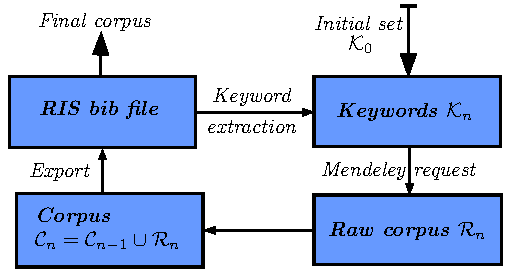
\includegraphics[width=0.7\textwidth]{/Users/Juste/Documents/ComplexSystems/CityNetwork/Docs/Papers/ECTQG2015/figures/schema_algo.pdf}
\caption{Global workflow of the algorithm. We provide also implementation details : catalog request is done through Mendeley API ; final state of corpuses are RIS files.}
\label{fig:algo}
\end{figure}




%%%%%%%%%%%%%%%%%%%%
\section{Results}
%%%%%%%%%%%%%%%%%%%%

%%%%%%%%%%%%%%%%%%%%
\subsection{Implementation}

\paragraph{General Implementation}
Because of the heterogeneity of operations required by the algorithm (references organization, catalog requests, text processing), it was found a reasonable choice to implement it in Java. Source code and binaries are available on the Github repository of the project\footnote{at \texttt{https://github.com/JusteRaimbault/CityNetwork/tree/master/Models/Biblio/AlgoSR/AlgoSRJavaApp}}.

\paragraph{Catalog Requests}
Given a set of keywords, we need to extract a corpus of articles from a bibliographical database. It has to be done automatically and records must have abstract record populated as text mining is mostly done on it. Therefore, it was chosen to use Mendeley reference manager software~\cite{mendeley} as it provide an open access to a flexible API that allows such catalog requests.


\paragraph{Natural Language Processing}
Keyword extraction is done through Natural Language Processing (NLP) techniques, following the workflow given in~\cite{chavalarias2013phylomemetic}. Although powerful and flexible libraries exist for current operations\footnote{see e.g. Java library by The Stanford Natural Language Processing Group at \texttt{http://nlp.stanford.edu/software/corenlp.shtml}, or Python library NLTK at \texttt{http://www.nltk.org/}.}, the elaborated workflow of the paper would be painful to implement and is furthermore already made available by the authors on the dedicated website of the \emph{CorText} project\footnote{\texttt{http://manager.cortext.net}}, platform with which we interacted automatically for the language processing step.


%%%%%%%%%%%%%%%%%%%%
\subsection{Convergence and Sensitivity Analysis}

It is not possible to formally show the convergence of the algorithm as it will depend on the unknown structure of request results and keywords extraction. We need thus to study empirically its convergence. For different initial request and many values of parameter $N_k$, we studied the number of references as a function of the iteration. Good convergence properties but various sensitivities to $N_k$ were found as presented in Fig. 2. We also studied the internal lexical consistence of final corpuses as a function of keyword number. As expected, small number gave more consistent corpuses, but the variability when increasing was reasonable, what gives a clue on the relevance of the approach that retrieves always stable corpuses.


\begin{figure}
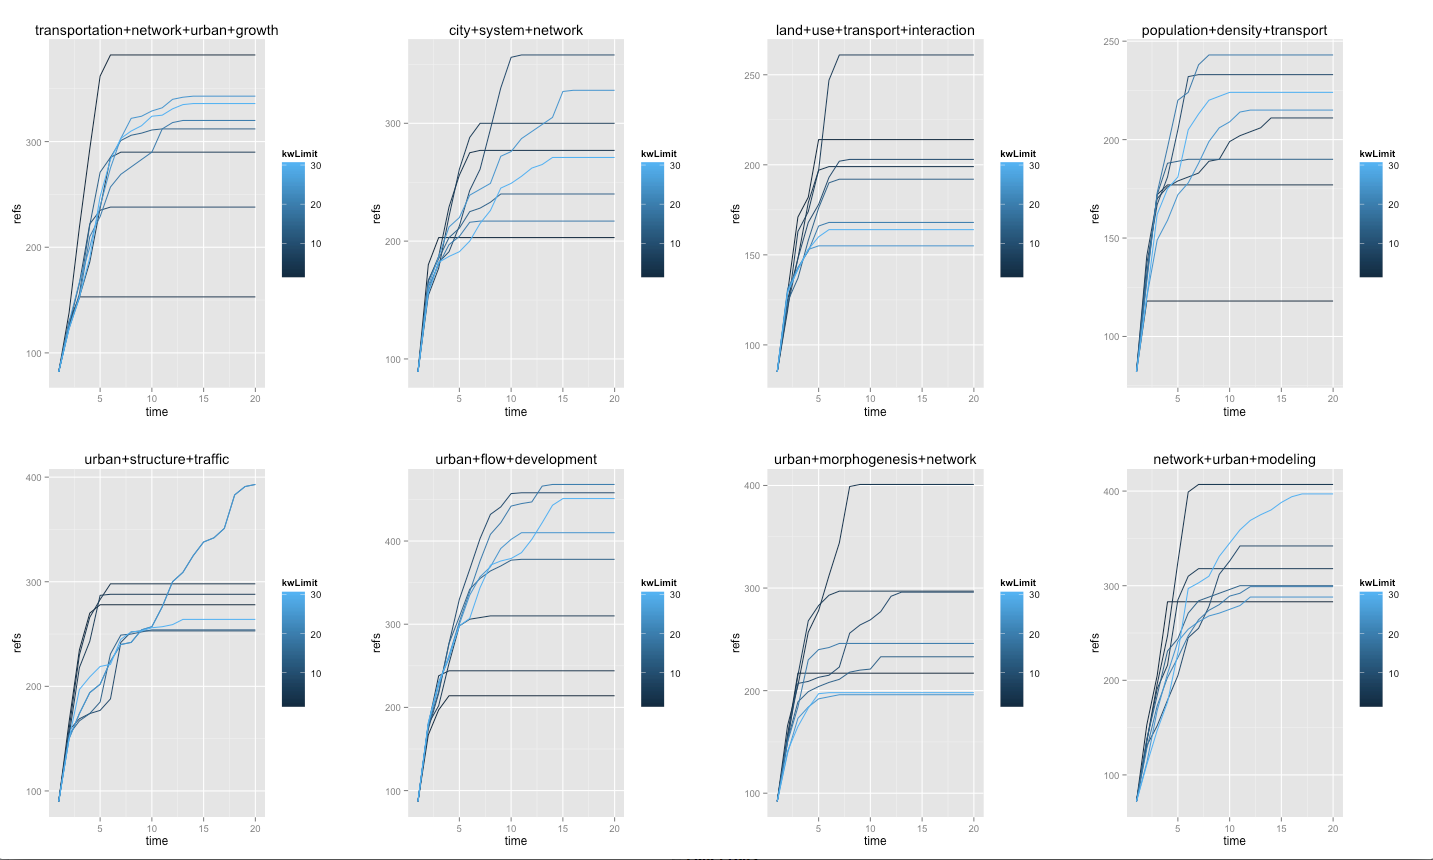
\includegraphics[width=0.68\textwidth]{figures/explo.png}
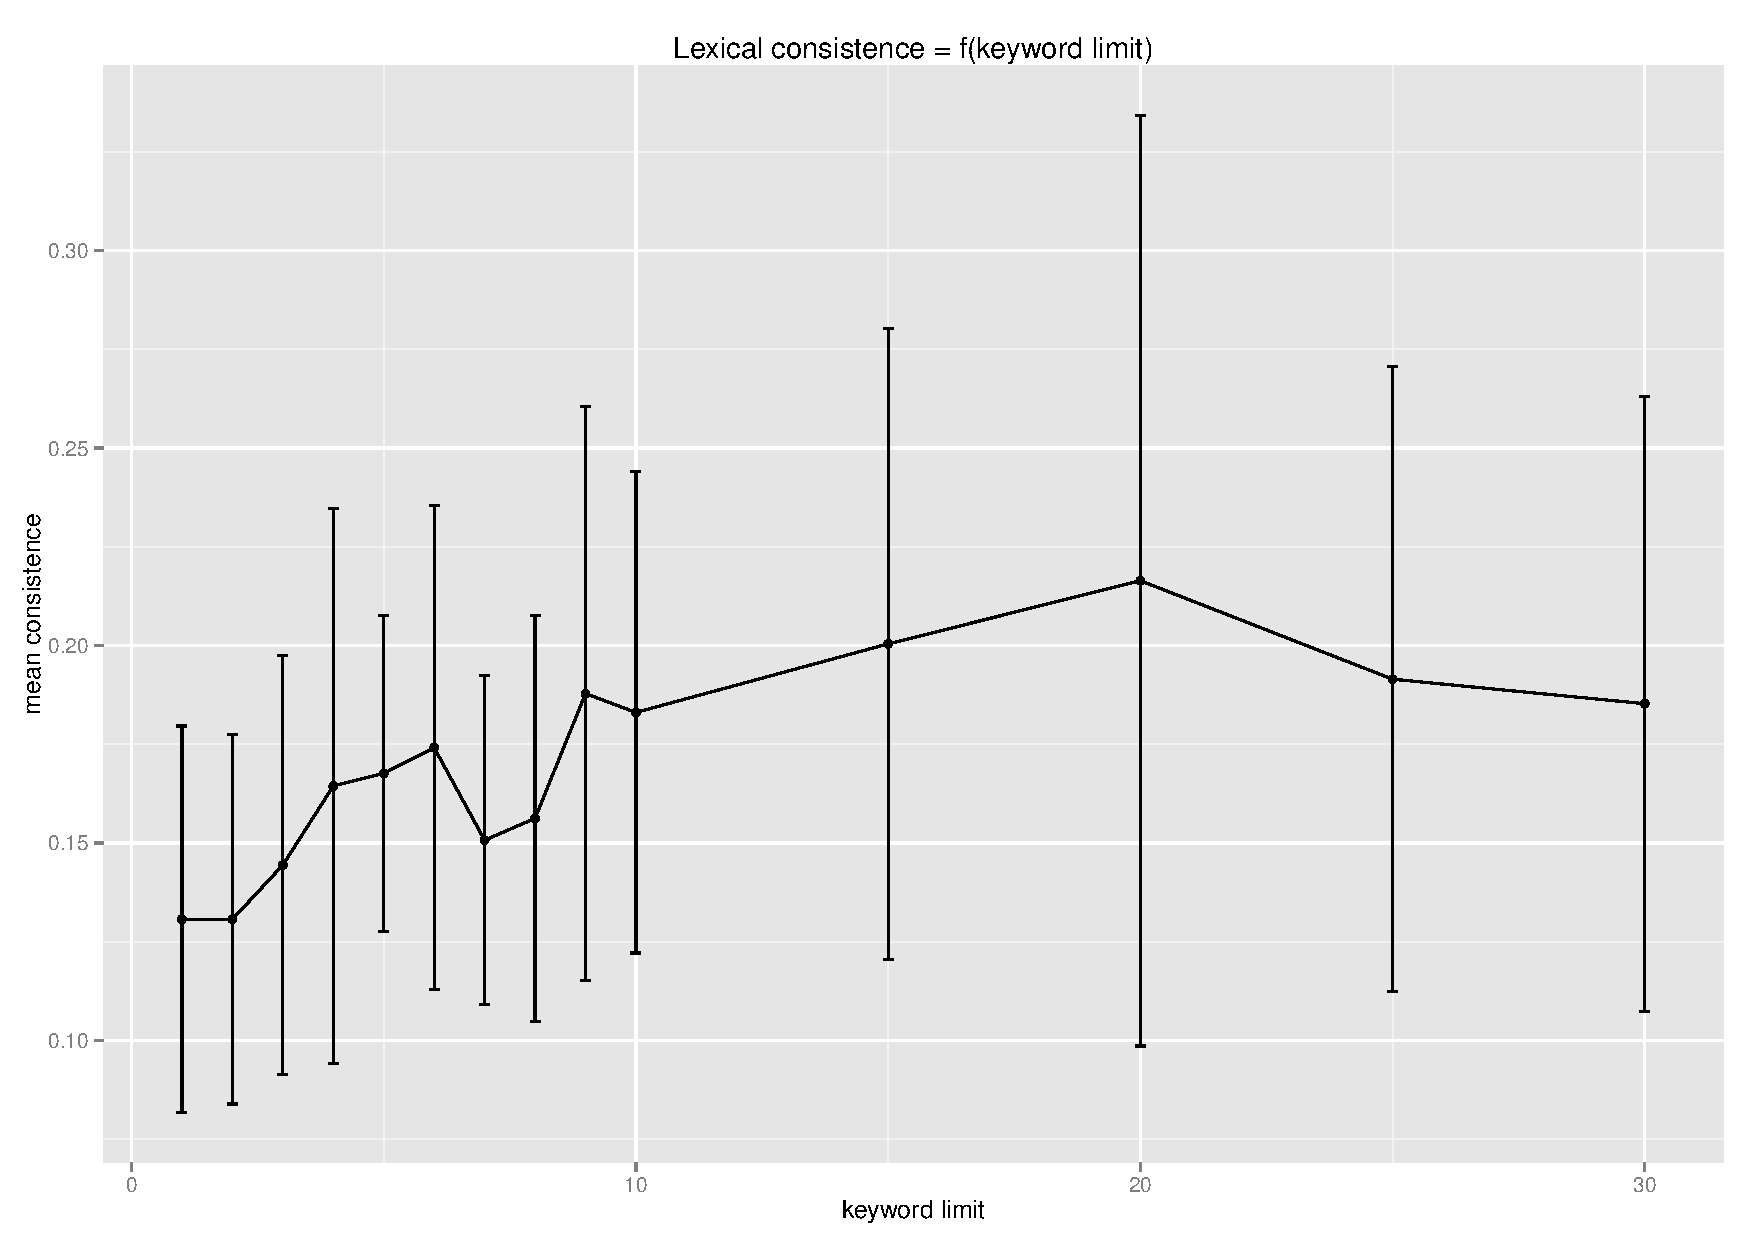
\includegraphics[width=0.3\textwidth,height=0.3\textheight]{figures/lexicalConsistence_MeanSd}
\caption{Convergence and sensitivity analysis.
\textit{Left : } Plots of number of references as a function of iteration, for various queries linked to our theme, for various values of $N_k$ (from 2 to 30). We obtain a rapid convergence for most cases, around 10 iterations needed. Final number of references appears to be very sensitive to keyword number depending on queries, what seems logical since encountered landscape should strongly vary depending on terms. \textit{Right : } Mean lexical consistence and standard error bars for various queries, as a function of keyword number. Lexical consistence is defined though co-occurrences of keywords by, with $N$ final number of keywords, $f$ final step, and $c(i)$ co-occurrences in references, $\kappa = \frac{2}{N(N-1)}\sum_{i,j \in \mathcal{K}_f}{|c(i)-c(j)|}$. The stability confirms the consistence of retrived corpuses.}
\end{figure}



%%%%%%%%%%%%%%%%%%%%
\subsection{Application}

Once the algorithm is validated, we can apply it to our question. We start from 5 different initial requests that were manually extracted from the various domains identified in the manual bibliography (that are \texttt{city+system+network}, \texttt{land+use+transport+interaction}, \texttt{network+urban+modeling}, \texttt{population+density+transport}, \texttt{transportation+network+urban+growth}). We take the weakest assumption on parameter $N_k=30$, as it should constrain less domains explorations and increase consistence of final results.

After having retrieved corpuses, we study their lexical distances as an indicator to answer our initial question. If they are indeed very far one from each other, it goes in the direction of the assumption made in section 2, i.e. that discipline self-centering may be at the origin of the non-existence of co-evolutive models. We show in Table 1 values of relative lexical proximity, that appear to be significantly low, what confirms our assumption.

\begin{table}
\centering
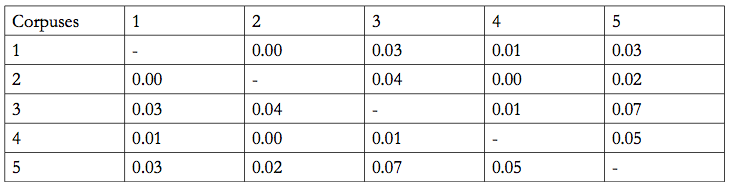
\includegraphics[width=\textwidth]{corpusesMatrix}
\caption{Symmetric matrix of lexical proximities between final corpuses, defined as the sum of overall final keywords co-occuring between corpuses, normalized by number of final keywords (100). We obtain very low values, confirming that corpuses are significantly far.}
\label{tab:res}
\end{table}


Further work is planned towards the construction of citation networks through an automatic access to Google Scholar that provides backward citations. The confrontation of inter-cluster coefficients on the citation network for the different corpuses with our lexical consistence results are an essential aspect of a further validation of our results.



%%%%%%%%%%%%%%%%%%%%
\section{Conclusion}
%%%%%%%%%%%%%%%%%%%%

The dramatic absence of models simulating the co-evolution of transportation networks and urban land-use, confirmed through a state-of-the-art covering many domain, may be due to the absence of communication between scientific disciplines studying different aspects of that problems. We have proposed an algorithmic method to give elements of answers through text-mining-based corpus extraction. First numerical results seem to confirm that assumption. However, such a work can not have a sense alone, but should come as a back-up for qualitative studies such as the one lead in~\cite{commenges:tel-00923682}, where free questionnaires with historical actors of modeling provide highly relevant information.



%%%%%%%%%%%%%%%%%%%%
%% Biblio
%%%%%%%%%%%%%%%%%%%%
\small

\bibliographystyle{apalike}
\bibliography{/Users/Juste/Documents/ComplexSystems/CityNetwork/Biblio/Bibtex/CityNetwork,/Users/Juste/Documents/ComplexSystems/Biblio/Culture/Culture/culture}


\end{document}
